
\documentclass[12pt,a4paper]{amsart}
% ukazi za delo s slovenscino -- izberi kodiranje, ki ti ustreza
\usepackage[slovene]{babel}
%\usepackage[cp1250]{inputenc}
\usepackage[T1]{fontenc}
\usepackage[utf8]{inputenc}
\usepackage{amsmath,amssymb,amsfonts}
\usepackage{url}
\usepackage{graphicx}
\usepackage{subcaption}
%\usepackage[demo]{graphicx}
%\usepackage[normalem]{ulem}
\usepackage[dvipsnames,usenames]{color}
\usepackage{hyperref}
\hypersetup{
     colorlinks   = true,
     citecolor    = gray
}

\graphicspath{ {./slike/} }
% ne spreminjaj podatkov, ki vplivajo na obliko strani
\textwidth 15cm
\textheight 24cm
\oddsidemargin.5cm
\evensidemargin.5cm
\topmargin-5mm
\addtolength{\footskip}{10pt}
\pagestyle{plain}
\overfullrule=15pt % oznaci predlogo vrstico


% ukazi za matematicna okolja
\theoremstyle{definition} % tekst napisan pokoncno
\newtheorem{definicija}{Definicija}[section]
\newtheorem{primer}[definicija]{Primer}
\newtheorem{opomba}[definicija]{Opomba}

\renewcommand\endprimer{\hfill$\diamondsuit$}


\theoremstyle{plain} % tekst napisan posevno
\newtheorem{lema}[definicija]{Lema}
\newtheorem{izrek}[definicija]{Izrek}
\newtheorem{trditev}[definicija]{Trditev}
\newtheorem{posledica}[definicija]{Posledica}


% za stevilske mnozice uporabi naslednje simbole
\newcommand{\R}{\mathbb R}
\newcommand{\N}{\mathbb N}
\newcommand{\Z}{\mathbb Z}
\newcommand{\C}{\mathbb C}
\newcommand{\Q}{\mathbb Q}

% ukaz za slovarsko geslo
\newlength{\odstavek}
\setlength{\odstavek}{\parindent}
\newcommand{\geslo}[2]{\noindent\textbf{#1}\hspace*{3mm}\hangindent=\parindent\hangafter=1 #2}

% naslednje ukaze ustrezno popravi
\newcommand{\program}{Finančna matematika} % ime studijskega programa: Matematika/Finan"cna matematika
\newcommand{\imeavtorja}{Eva Ozebek\\ Jan Kolenc} % ime avtorja
\newcommand{\imementorja}{prof. dr. Riste Škrekovski} % akademski naziv in ime mentorja
\newcommand{\naslovdela}{Minimum vertex cover}
\newcommand{\letnica}{2019} %letnica




\begin{document}

% od tod do povzetka ne spreminjaj nicesar
\thispagestyle{empty}
\noindent{\large
UNIVERZA V LJUBLJANI\\[1mm]
FAKULTETA ZA MATEMATIKO IN FIZIKO\\[5mm]
\program\ -- 1.~stopnja}
\vfill

\begin{center}{\large
\imeavtorja\\[2mm]
{\bf \naslovdela}\\[10mm]
Projekt v povezavi z OR\\[1cm]}

\end{center}
\vfill

\noindent{\large
Ljubljana, \letnica}
\pagebreak

\thispagestyle{empty}
\hypersetup{linkcolor = black}
\tableofcontents
\pagebreak

\section{Navodilo}


Define the Minimum vertex cover problem as an ILP and solve it for some examples. Also, solve the LP relaxation of this problem for the same cases. Note that its LP relaxation gives a solution that is at most twice bigger than the optimal one. Compare the sizes of both solutions on various graphs to verify this and determine experimentally by how much, in average, the LP relaxation solution is larger than the optimal one. Finally, present and implement a greedy algorithm and the one using the maximal matching described in the book below. Test the sizes of these three solutions. Try to determine for how large graphs each of these algorithms is tractable.

\newpage
\section{Uvod}

Najina naloga je, da problem najmanjšega vozliščnega pokritja predstaviva kot problem ILP, LP relaksacije ter požrešnega algoritma. Pri tem bova algoritme preverila za 1000 različnih primerov grafov, ki imajo naključno med 5 in 100 vozlišč in naključnih povezav. Primerjala bova rezultate različnih algoritmov, kjer naju bo še posebej zanimala velikost rešitve oz. v najinem primeru velikost vrnjene množice.
Najine algoritme bova testirala na podatkih, ki jih bova generirala sama.

\hspace*{\fill} % it's important not to leave blank lines before and after this command

Problem \textit{najmanjšega vozliščnega pokritja}  je eden izmed osnovnih problemov pokrivanja. Kot pove že ime samo, je problem definiran s pomočjo teorije grafov. Gre za pokrivanje povezav grafa z vozlišči, t.j. za iskanje najmanjše podmnožice vozlišč grafa, ki vsebuje vsaj eno krajišče vsake povezave grafa.

\hspace*{\fill} % it's important not to leave blank lines before and after this command

Pri programiranju in pisanju algoritma sva se odločila za program Sage, saj je le-ta za najino nalogo najbolj primeren.

\newpage

\begin{figure*}[ht]
\centering
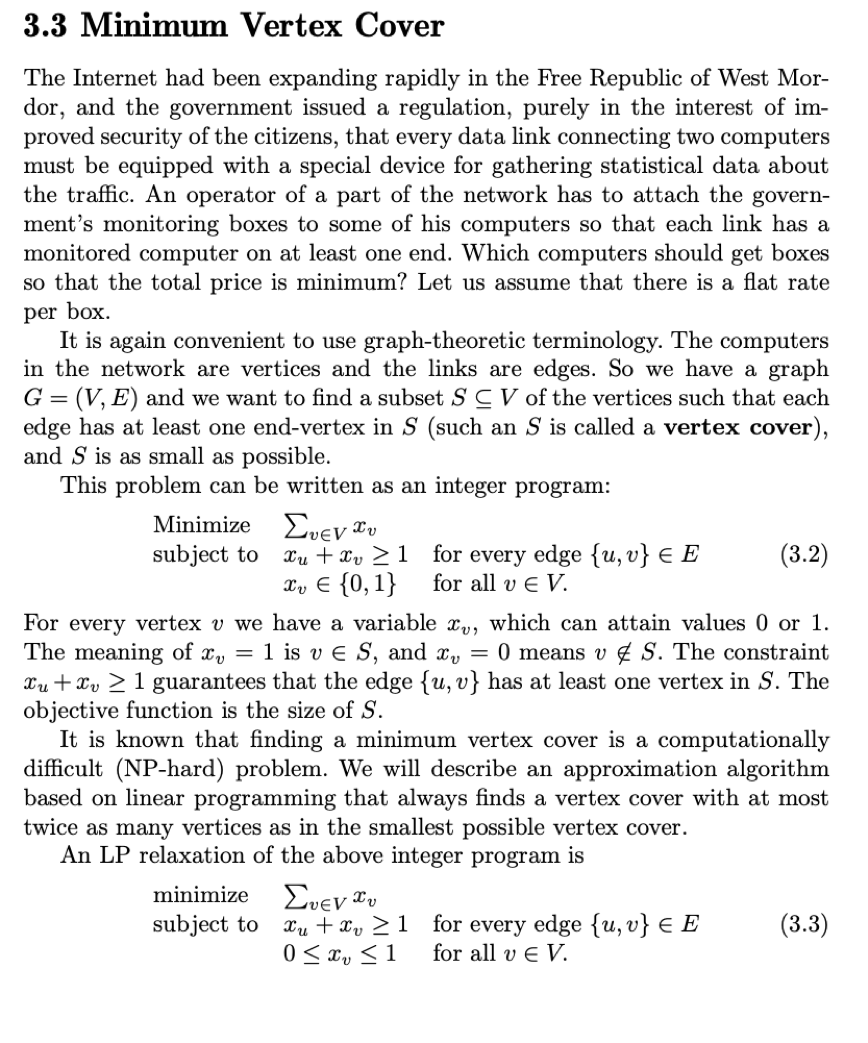
\includegraphics[width=1\textwidth]{Picture1.png}
\end{figure*}

\newpage

\begin{figure*}[ht]
\centering
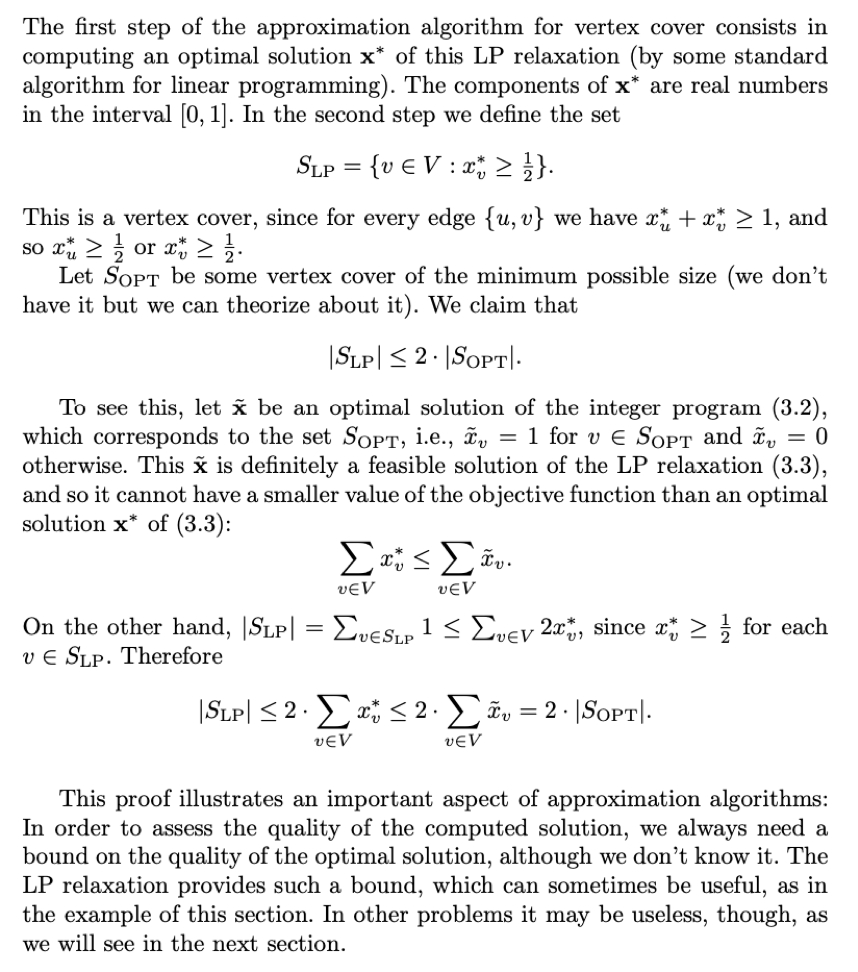
\includegraphics[width=1\textwidth]{Picture2.png}
\end{figure*}


\newpage

\begin{figure*}[ht]
\centering
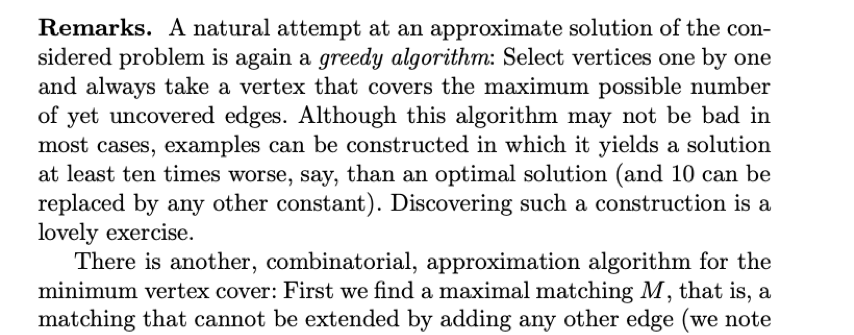
\includegraphics[width=1\textwidth]{Picture3.png}
\end{figure*}

\begin{figure*}[ht]
\centering
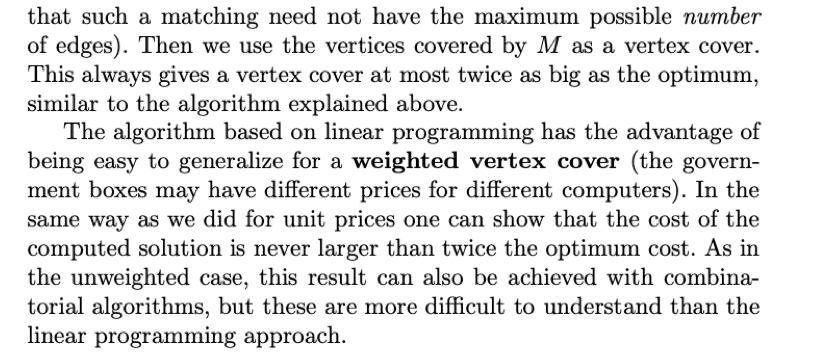
\includegraphics[width=1\textwidth]{Picture4.png}
\end{figure*}

%---------------------OPIS DELA- SCREENSHOTI --------------------

\newpage

\section{Opis dela}
\

\subsection{Generiranje grafov}
\
\\
\\
Najprej sva definirala funkcijo testiranje, ki vzame argumente \textit{a} (število različnih velikosti grafov), \textit{b} (število grafov iste velikosti), \textit{c} (največje možno število vozlišč), kar bomo uporabili pri generaciji grafov. Funkcija si na začetku shrani tudi 3 števce in sicer: koliko grafov smo že pregledali, seštevek koeficientov razlik - razlika velikosti rešitev ILP in LP ter razlika velikosti rešitev greedy in max matching. 




\begin{figure*}[ht]
\centering
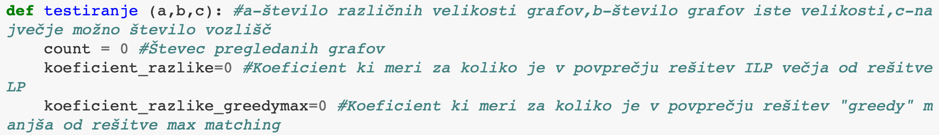
\includegraphics[width=1\textwidth]{Screen2.png}
\end{figure*}

Ko izžrebamo število vozlišč moramo še 10x žrebati število povezav. Generirala sva naključno število vozlišč in povezav, kjer sva število povezav morala omejiti (da ne presegajo števila povezav polnega grafa na c vozliščih), od tu izraz c*(c - 1)/2. Ko se vozlišča in povezave naključno izberejo, na vsakem izmed 1000 korakov dobimo graf na katerem uporabljamo algoritme.



\begin{figure*}[ht]
\centering
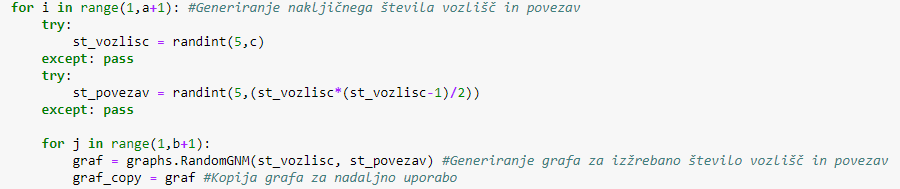
\includegraphics[width=1\textwidth]{Screen3.png}
\end{figure*}

\newpage

\subsection{Požrešni algoritem}
\
\\
\\
Definirala sva požrešni algoritem, ki sledi reševanju problemov heuristiki izbire lokalno optimalne izbire na vsaki stopnji z namenom poiskati globalni optimum. Le-ta vsakič vzame vozlišče z največ povezavami in ta vozlišča shranjuje v seznam. 

Torej, ko imamo vozlišče z največ povezavami, te povezave odstranimo in to ponavljamo tako dolgo, dokler v grafu ni več nobenih povezav. Ta izbrana vozlišča so vertex cover. Hkrati sva uporabila implementiran algoritem za maximum matching, ki nam vrne povezave, zato na koncu pomnožimo z 2, saj nas zanima število vozlišč. Kot lahko opazimo je naša rešitev seznam, dolžina seznama pa predstavlja velikost rešitve. 

\begin{figure*}[ht]
\centering
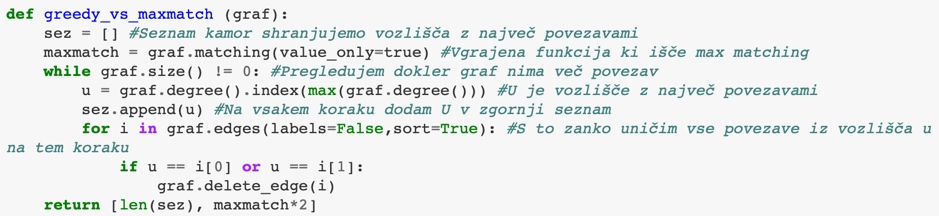
\includegraphics[width=1\textwidth]{Screen1.png}
\end{figure*}




\subsection{Celoštevilski linearni program}
\
\\
\\
Ko imamo generiran graf, le-tega "spustimo" čez vse 4 algoritme. 
ILP \textit{integer linear program } uporablja samo ničle in enke (cela števila na zaprtem intervalu od 0 do 1), zato nastavimo \textit{binary = True}. Z \textit{set objective} določimo kaj želimo maksimizirati pri linearnih programih. Nato omejitve (constraints) nastavimo tako, da je vsaka povezava v grafu všteta vsaj enkrat. Kot lahko opazimo v zadnji vrstici, nam vozlišča dajo value. 



\begin{figure*}[ht]
\centering
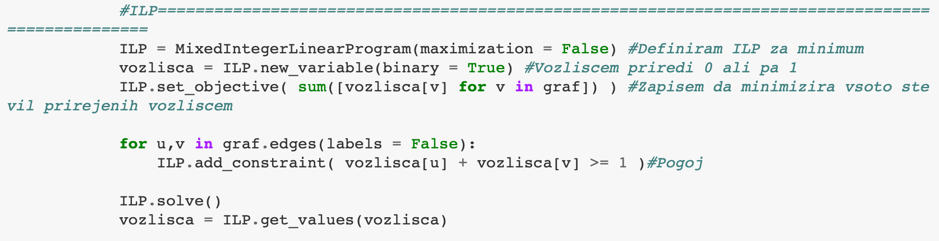
\includegraphics[width=1\textwidth]{Screen4.png}
\end{figure*}

\newpage

\subsection{Relaksacija celoštevilskega na linearni program}
\
\\
\\
Tukaj se ne ukvarjamo več z celimi števili, zato nastavimo \textit{real = True}. Realna števila sva omejila na interval od 0 od 1, nastavila sva iste pogoje in enak objective.

Ker uporabimo pogoj da mora biti vsota vozlišč večja ali enaka ena, vemo da mora biti posamezno vozlišče večje ali enako eni polovici. 


\begin{figure*}[ht]
\centering
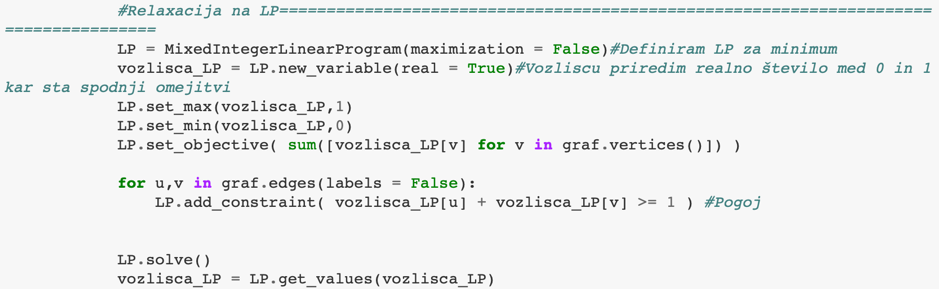
\includegraphics[width=1\textwidth]{Screen5.png}
\end{figure*}


\newpage

\subsection{Rezultati}
\
\\
\\
Na tej točki upoštevamo \textit{greedy}, ki sva ga definirala zgoraj. Print sprinta obe rešitvi (greedy in maxmatch) hkrati, zato potem pogledamo koeficient razlike pri vsaki posebej in ga prištejemo k števcu za ta koeficient.  Na koncu zdelimo velikosti, da vidimo koliko so se razlikovali v povprečju. 


\begin{figure*}[ht]
\centering
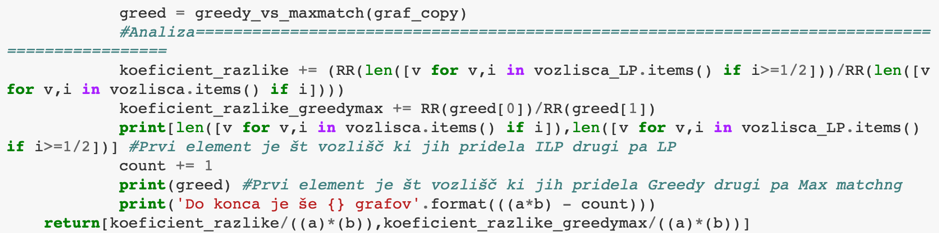
\includegraphics[width=1\textwidth]{Screen6.png}
\end{figure*}

\begin{figure*}[ht]
\centering
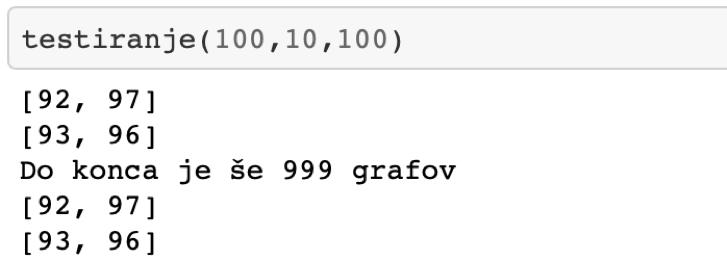
\includegraphics[width=.6\textwidth]{Screen7.png}
\end{figure*}



\begin{figure*}[ht]
\centering
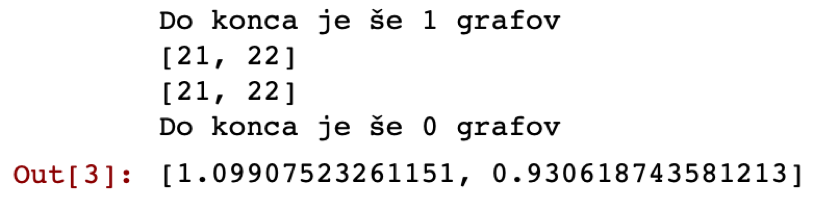
\includegraphics[width=.7\textwidth]{Screen8.png}
\end{figure*}


\newpage



\section{Zaključek}

V najini analizi sva se, kot omenjeno že prej, osredotočila na 1000 primerov, ki sva jih generirala sama. Najprej sva definiranim grafom naključno izbrala med 5 in 100 vozlišč, nato pa dodala še naključne povezave.

\hspace*{\fill} % it's important not to leave blank lines before and after this command


Tekom analize sva uporabljala sledeče algoritme:
\begin{itemize}
\item ILP
\item LP
\item Požrešni algoritem
\item Maximal matching

 \end{itemize}

 \hspace*{\fill} % it's important not to leave blank lines before and after this command


V najini analizi sva imela težave pri omejevanju števila povezav, saj le-teh najprej nisva omejila, kjer se je pri večjih grafih posledično zatikalo oz. trajalo dlje. 

Po koncu najinega eksperimenta na 1000 grafih, lahko povzameva, da so rezultati kot pričakovani. 
Ta problem je NP-težek, kar pomeni, da zanj domnevno ne obstaja polinomsko časovno omejen algoritem. 

Pri algoritmu ILP smo vedno dobili manjše rešitve kot pri drugih algoritmih, za kar lahko rečemo, da je ta algoritem bolj učinkovitejši od drugih.




\hspace*{\fill} % it's important not to leave blank lines before and after this command



%VIRI SO NAVEDENI :)

\newpage
\begin{thebibliography}{}


\bibitem{teorija}
J.~Matoušek in B.~Gartner, \emph{Understanding and Using Linear Programming}


\bibitem{teorija}
 J.~Mihelič, \emph{Algoritem za problem najmanjšega vozliščnega pokritja}, [ogled 18.~11.~2019], dostopno na \url{https://www.researchgate.net/publication/308929074_Algoritmi_za_problem_najmanjsega_vozliscnega_pokritja?fbclid=IwAR0n6CzQluY3ZFM6g2-yQ_fPLnUiT8zrb78S_o3VUwjmf7F-_DNQzxHVqb0}




\end{thebibliography}{}

\end{document}
